\label{chap:intro}

\section{Background}
\label{sec:intro-background}
A household robot that is asked to ``find something to heat my lunch'' must solve two problems at once. It must
ground an open-ended instruction in what its camera sees, deciding that a microwave or a toaster satisfies the
request, and it must move through a room it does not know until it reaches that object. The two problems have
historically been studied by different communities with different tools.

Classical mobile robotics solves the second problem well. Occupancy grids~\cite{elfes1989occupancy} turn range
measurements into a probabilistic map of free and occupied space, frontier exploration~\cite{yamauchi1997frontier}
drives the robot toward the boundary between known and unknown space, and graph search such as A*~\cite{hart1968astar}
computes collision-free paths on the map. These components are interpretable, need no training data, and are
reliable enough to be the default in deployed robots~\cite{thrun2005probabilistic}. They know where the robot can
go, but not where a ``kettle'' or ``something to sit on'' is.

The first problem, grounding language in perception, was for a long time restricted to fixed object categories.
Vision-language models (VLMs) trained on web-scale image-text pairs changed this: contrastive models and
open-vocabulary detectors recognize objects named in free text~\cite{radford2021clip,minderer2022owlvit,liu2024groundingdino},
and generative VLMs answer questions about images and localize objects described in words~\cite{bai2025qwen25vl,bai2025qwen3vl}.

Multimodal large language models (MLLMs) have since been used as complete embodied agents. EmbodiedBench evaluates
such agents on standard tasks through a common action interface~\cite{yang2025embodiedbench}. In its navigation
benchmark, EB-Navigation, the agent receives an instruction and a first-person camera image and must come within
1\,m of the described object within 20 steps. The benchmark's own agent gives the model every role. At each step
the model reads the current image and the text history of its previous actions, describes what it sees, reasons
about where the target is, and writes a plan of the next actions.

\section{Motivation}
\label{sec:intro-motivation}
The success of this design tracks model size. GPT-4o succeeds in 57.7\% of the EB-Navigation episodes and
InternVL3-78B in 53.7\%, while models of 7--8B reach 20.3--29.3\% overall and 0--5\% on the Long-horizon subset, in
which the target starts behind the agent~\cite{yang2025embodiedbench}. A tenfold larger model of the same family adds
\nScaleQwen--\nScaleIntern{} percentage points.

The gap matters because a robot has good reasons to use a small local model. A model that runs on the robot's own
computer or on a consumer GPU works without a network connection, answers with a predictable latency, keeps camera
images of a private home on the device, and costs nothing per query. The models that fit these constraints today
have a few billion parameters and are quantized to 4 or 8 bits~\cite{lin2024awq}. A robot that must rely on such a
model cannot adopt the agent designs that work with frontier models, because those designs fail with small models.

The question this thesis pursues is whether the failure is a property of small models or a property of how they are
used. If small models fail because they cannot see well enough, the only remedies are larger models or task-specific
training. If they fail because the agent asks them to do something other than seeing, a different agent may make
them work as they are.

\section{Problem statement}
\label{sec:intro-problem}
Existing remedies keep the model in charge of the plan. Training-free agents surround it with memory, reflection,
skill libraries, scene graphs, or tools~\cite{lee2026emho,ma2026brainmem,zhou2026enabling,huang2025esca,ju2026embodiskill},
but the model still reads that context and writes the plan, and the reported gains rely on models of 8B parameters up
to frontier scale. Fine-tuned agents adapt a 4B model to the task~\cite{xie2026sva,jang2026musix} with training data
and compute, and remain below 60\% on EB-Navigation. Modular object-navigation systems keep a metric map and a
planner~\cite{gadre2022cows,yokoyama2023vlfm,yin2024online}, but they rely on dedicated detectors for fixed
categories, often together with a large language model that decides where to explore.

The problem addressed in this thesis is therefore the following: given a small, frozen, quantized VLM that runs
locally, build an embodied agent that follows open navigation instructions as well as agents built on much larger
models, without task-specific training.

\section{Research questions}
\label{sec:intro-rq}
The thesis is organized around three research questions.
\begin{description}
\item[RQ1. Why do small VLMs fail as navigation agents?] A small VLM may fail because it cannot recognize the
target, because it cannot plan motion, or because it cannot keep track of spatial state across steps. The thesis
separates these causes with controlled experiments on the same test episodes (\cref{chap:diagnosis}).
\item[RQ2. What should an agent built around a small VLM look like?] Once the cause is known, the agent should give
the model only the role it can fill. The thesis asks which components such an agent needs and which of them carry
the gain (\cref{chap:method,sec:exp-modular,sec:exp-ablation}).
\item[RQ3. How close does this agent come to agents built on larger models?] The thesis compares the agent with the
benchmark's agent and a modular agent that use the same model, with published agents built on larger
models, without a depth sensor, with a smaller model, and on a second benchmark that requires an explicit stop
(\cref{chap:experiments}).
\end{description}

\section{Scope}
\label{sec:intro-scope}
The thesis studies object-goal navigation from natural-language instructions in indoor simulated scenes. The main
benchmark is EB-Navigation, in which each episode takes place in one AI2-THOR room~\cite{kolve2017ai2thor}; RoboTHOR
ObjectNav~\cite{deitke2020robothor} adds multi-room apartments, longer episodes, and an explicit stop decision. The
agent uses one frozen open VLM of 3--4B parameters, quantized to 4 bits and served on a single 8\,GB GPU, and no
component is trained for the task. Manipulation, multi-step tasks, and deployment on a physical robot are outside
the scope of the experiments and are discussed as future work (\cref{chap:conclusions}).

\section{Approach}
\label{sec:intro-approach}
The thesis first diagnoses the failure. Motion planning is not the bottleneck: a geometric planner given the true
target position solves \nOracle\% of the EB-Navigation test episodes. Recognition is imperfect but usable: from a
single view, Qwen3-VL-4B~\cite{bai2025qwen3vl} places a box on a visible target whose category the instruction names
or implies in \nProbeThreeCommon--\nProbeThreeBase\% of the cases. The failure lies in between. Asked for a plan at
every step, the model must carry where the target was and which way it faces through generated text, and nothing
checks this text against the world. Prompted agents therefore lose targets they have seen, collide with furniture,
and never turn toward a target behind them.

This diagnosis points to a different division of labor: a small VLM is a good semantic sensor and a poor state
keeper. The thesis therefore builds the agent around the model rather than inside it (\cref{fig:arch}). The
Semantic-to-Metric (\ours) agent has three parts. \emph{Perception} asks the VLM two questions per frame, whether the
target is visible and where it is in the image, and checks a magnified crop only when the answer is weak.
\emph{Memory} lifts each answer with depth and pose into a metric target hypothesis, accumulates evidence only from
distinct viewpoints, and discards a hypothesis that reaching it shows to be a look-alike. \emph{Action} commits to a
confident hypothesis, inspects a weak one in view, and otherwise looks around and explores, while an occupancy-map
planner computes every move. Each part removes one diagnosed failure: the memory keeps a seen target,
the map prevents collisions, and the look-around finds a target behind the agent. The model never plans and never
sees the history.

\begin{figure}[htbp]
\centering
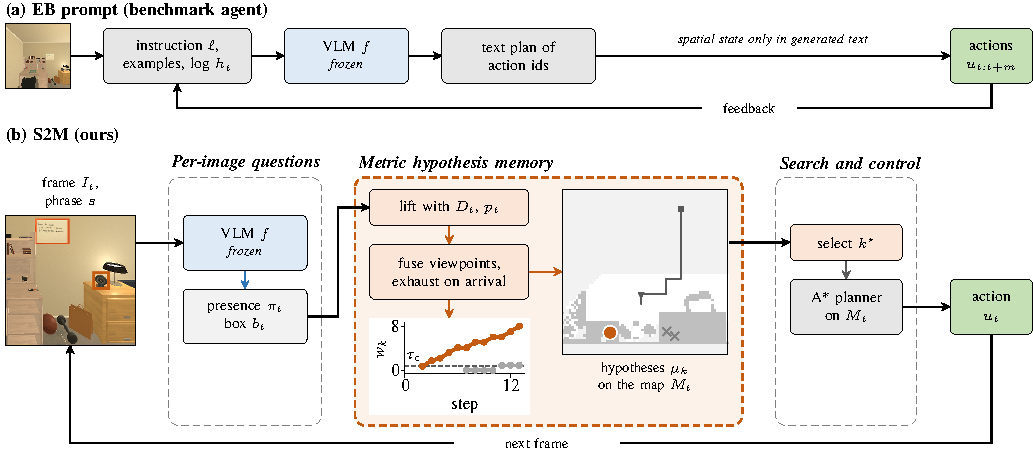
\includegraphics[width=\linewidth]{figures/fig_arch.pdf}
\caption[The benchmark's agent and the Semantic-to-Metric agent]{\textbf{(a)}~The EB prompt maps the image $I_t$,
the instruction $\ell$, and the history $h_t$ to a text plan $u_{t:t+m}$ with the VLM $f$. \textbf{(b)}~\ours asks
$f$ for the presence $\pi_t$ and box $b_t$ of the phrase $s$, lifts them with depth $D_t$ and pose $p_t$ into
hypotheses $\mu_k$ with evidence $w_k$, selects $k^\star$, and plans $u_t$ on the map $M_t$. Thumbnails: a
Long-horizon test episode, with the VLM's box on the target, the evidence of the target (orange) rising to ten times
the commit threshold $\tau_\mathrm{c}$ while two look-alikes (grey) stay near or below it, and the map with the path,
the target (orange), and the look-alikes ($\times$). Blue: the frozen VLM; orange: the hypothesis memory of \ours and
the selection that reads it.}
\label{fig:arch}
\end{figure}

The agent is evaluated on the full EB-Navigation test set and the full RoboTHOR validation split with two model
generations, repeated runs, and paired statistics. Changing the model's role moves it further than scaling it. With
Qwen3-VL-4B at 4-bit, \ours succeeds in \nSThree\% of the EB-Navigation test episodes, \nGainThree{} percentage points
more than the benchmark's agent with the same model, as much as the tenfold scale-up from InternVL3-8B to 78B gives,
and it closes \nGapClosed\% of the gap to the oracle planner. Each step takes \nSecS\,s instead of \nSecEB\,s, because
the model answers two short questions instead of writing a plan.

\section{Contributions}
\label{sec:intro-contrib}
The thesis makes the following contributions.
\begin{enumerate}
\item \textbf{A diagnosis of small-VLM navigators.} Controlled experiments on the same test episodes show that small
VLMs fail as navigation agents because they must keep spatial state in generated text, not because they cannot
recognize the target or plan a path. The diagnosis yields four predictions, all of which the experiments confirm.
\item \textbf{The VLM as a sensor, not a planner.} \ours inverts the control of MLLM agents: a metric controller asks
the VLM only questions that the current image can settle, and the VLM never sees the history, the map, or the plan.
\item \textbf{Evidence fusion for a generative sensor.} A metric hypothesis memory accumulates the model's presence
and box answers over distinct viewpoints and discards look-alikes on arrival, which turns unreliable single
answers into a stable target. A modular agent that is \ours without fusion and the crop check, and so acts on single-view
answers with the same model and planner, trails \ours by \nSOverMod{} percentage points.
\item \textbf{Navigation from RGB alone.} A per-frame ground-plane scale for monocular depth raises RGB-only success
from \nRGBGlobal\% with a global scale to \nRGBThree\%, within \nGapRGBAbs{} percentage points of a depth sensor.
\item \textbf{A training-free 4B agent that rivals far larger ones.} From RGB alone, \ours is above GPT-4o, both fine-tuned
4B agents, and \nNTrainFreeBelowRGB{} of \nNTrainFree{} training-free agents built on 8B to frontier-scale models; with a depth sensor, changing the
model's role gives as much as a tenfold larger model. With Qwen2.5-VL-3B~\cite{bai2025qwen25vl}
its gain over the benchmark's agent grows to \nGainTwo{} percentage points, and on RoboTHOR it reaches \nRoboSR\%
success, above ten published zero-shot methods.
\end{enumerate}

\section{Thesis organization}
\label{sec:intro-outline}
\Cref{chap:literature} reviews embodied navigation, zero-shot object navigation, MLLM agents, and the methods for
memory, verification, and geometry on which \ours builds. \Cref{chap:prelim} defines the task, the benchmarks, the
metrics, the models, and the statistical protocol. \Cref{chap:diagnosis} diagnoses why a small VLM fails when it is
prompted as the benchmark's agent and derives four predictions. \Cref{chap:method} presents \ours, and
\cref{chap:experiments} tests the predictions and analyses the agent. \Cref{chap:conclusions} answers the research
questions, discusses the findings and limitations, and outlines future work. \Cref{app:impl} lists the prompts,
parameters, and serving settings, and \cref{app:results} gives the evaluation protocol and additional results.
